\documentclass[12pt]{article}

\usepackage{amsmath}

\usepackage{graphicx}

\usepackage{hyperref}

\usepackage{xcolor}

\usepackage{amsmath} % for 'pmatrix' environment

\usepackage{listings} %code representation

\usepackage{trfsigns} %transformationszeichen

\usepackage{float} %floating images

\usepackage{subfig} %images next to one another

\usepackage{amssymb} %arrows

\usepackage{pdfpages} %add pdf to latex file

\renewcommand*\contentsname{Inhaltsverzeichnis} % rename table of content

\usepackage{fancyhdr} %header and footer

% colored \pm
\usepackage{stackengine,xcolor}
\def\cpm{\mathbin{\ensurestackMath{\abovebaseline[-3.4pt]{%
				\stackunder[-3.5pt]{\color{green!70}+}{\color{red}-}}}}}

\usepackage[utf8]{inputenc}

\begin{document}
	\begin{titlepage}
		\centering
		\vspace{1cm}
		{\scshape\LARGE Hochschule Luzern \\ Technik und Architektur \par}
		\vspace{1cm}
		{\scshape\Large Bachelor Thesis\par}
		\vspace{1.5cm}
		{\huge\bfseries Entwicklung einer PCB zur Analyse von Umgebungslärm\par}
		\vspace{2cm}
		{\Large\itshape Stefano Nicora\par}
		
		\vfill
		
		% Bottom of the page
		{\large 7. Juni 2024\par}
	\end{titlepage}
	\tableofcontents
	
	%to do: add footer and header
	
	\newpage
	\section{Einleitung}
	\subsection{Ausgangslage}
	Die Firma hEar hat es sich zum Ziel gesetzt, gegen \color{red}TODO\color{black}. Dazu wurde in der Masterarbeit von Sophie Mia Willener eine Marktanalyse durchgeführt, sowie ein erster Prototyp gebaut. Dieser Prototyp ist jedoch noch unhandlich und nicht für den Massenmarkt geeignet. 
	\subsection{Ziele}
	Das Ziel dieser Arbeit ist es, in einem ersten Schritt, auf Basis des vorhandenen Prototypen, ein funktionales, kompaktes und portables Schalldruckpegel-Messgerät zu entwickeln. Dabei sollen folgende Rahmenbedingungen zwingend eingehalten werden:
	\begin{itemize}
		\item Die Laufzeit des Gerätes soll mindestens 12 Stunden betragen.
		\item Das Gerät wird mit einem Akku betrieben. Dieser wird via eines USB-C-Anschlusses aufgeladen.
		\item Der Schalldruckpegel wird mit einem MEMS-Mikrofon aufgezeichnet.
		\item Die Messdaten werden in regelmässigen Abständen auf dem Gerät gespeichert.
		\item Das Gerät verfügt über eine BLE-Schnittstelle um die Messdaten drahtlos an ein Zielgerät zu übertragen.
		\item Der aktuelle Schalldruckpegel wird auf der Vorderseite des Gerätes visuell dargestellt.
	\end{itemize}
	In einem zweiten Schritt, wird das Gerät kalibriert und dessen Qualität mit auf dem Markt bereits vorhandenen Geräten verglichen.
	
	\newpage
	\section{Mikrofon}
	\subsection{Grundlagen}
	\subsubsection{MEMS}
	
	\subsubsection{I2S}
	Inter-Integrated Sound (I²S) bezeichnet eine Bus-Schnittstelle, welche von Philips zur Übertragung von digitalen Audiosignalen entwickelt wurde. Ähnlich wie I²C (Inter-Integrated Circuit) wird die Schnittstelle jedoch nur innerhalb des Gerätes verwendet. Dabei werden drei Pins zwischen Sender (hier das Mikrofon) und dem Empfänger (hier der Mikrocontroller) benötigt:
	\begin{itemize}
		\item \textbf{SCK} \quad (Serial Clock) \\
		Generiert die Taktrate, welche gleichzeitig die Datenrate der Übertragung definiert. Die Taktrate wird vom Master (hier der Mikrocontroller) vorgegeben.
		\item \color{green}\textbf{WS}\color{black} \quad (Word Select) \\
		Gibt vor, welcher Audiokanal (R, L) übertragen werden soll. Dies ermöglicht es, entweder ein Stereo-Signal oder zwei Mono-Signale wie zum Beispiel zwei Mikrofone zu übertragen.
		\item \color{red}\textbf{SD}\color{black} \quad (Serial Data)
		Beinhaltet den eigentlichen Datenstream mit der Datenrate definiert durch SCK und der Länge definiert durch WS.
	\end{itemize}
	\begin{figure}[H]
		\centering
		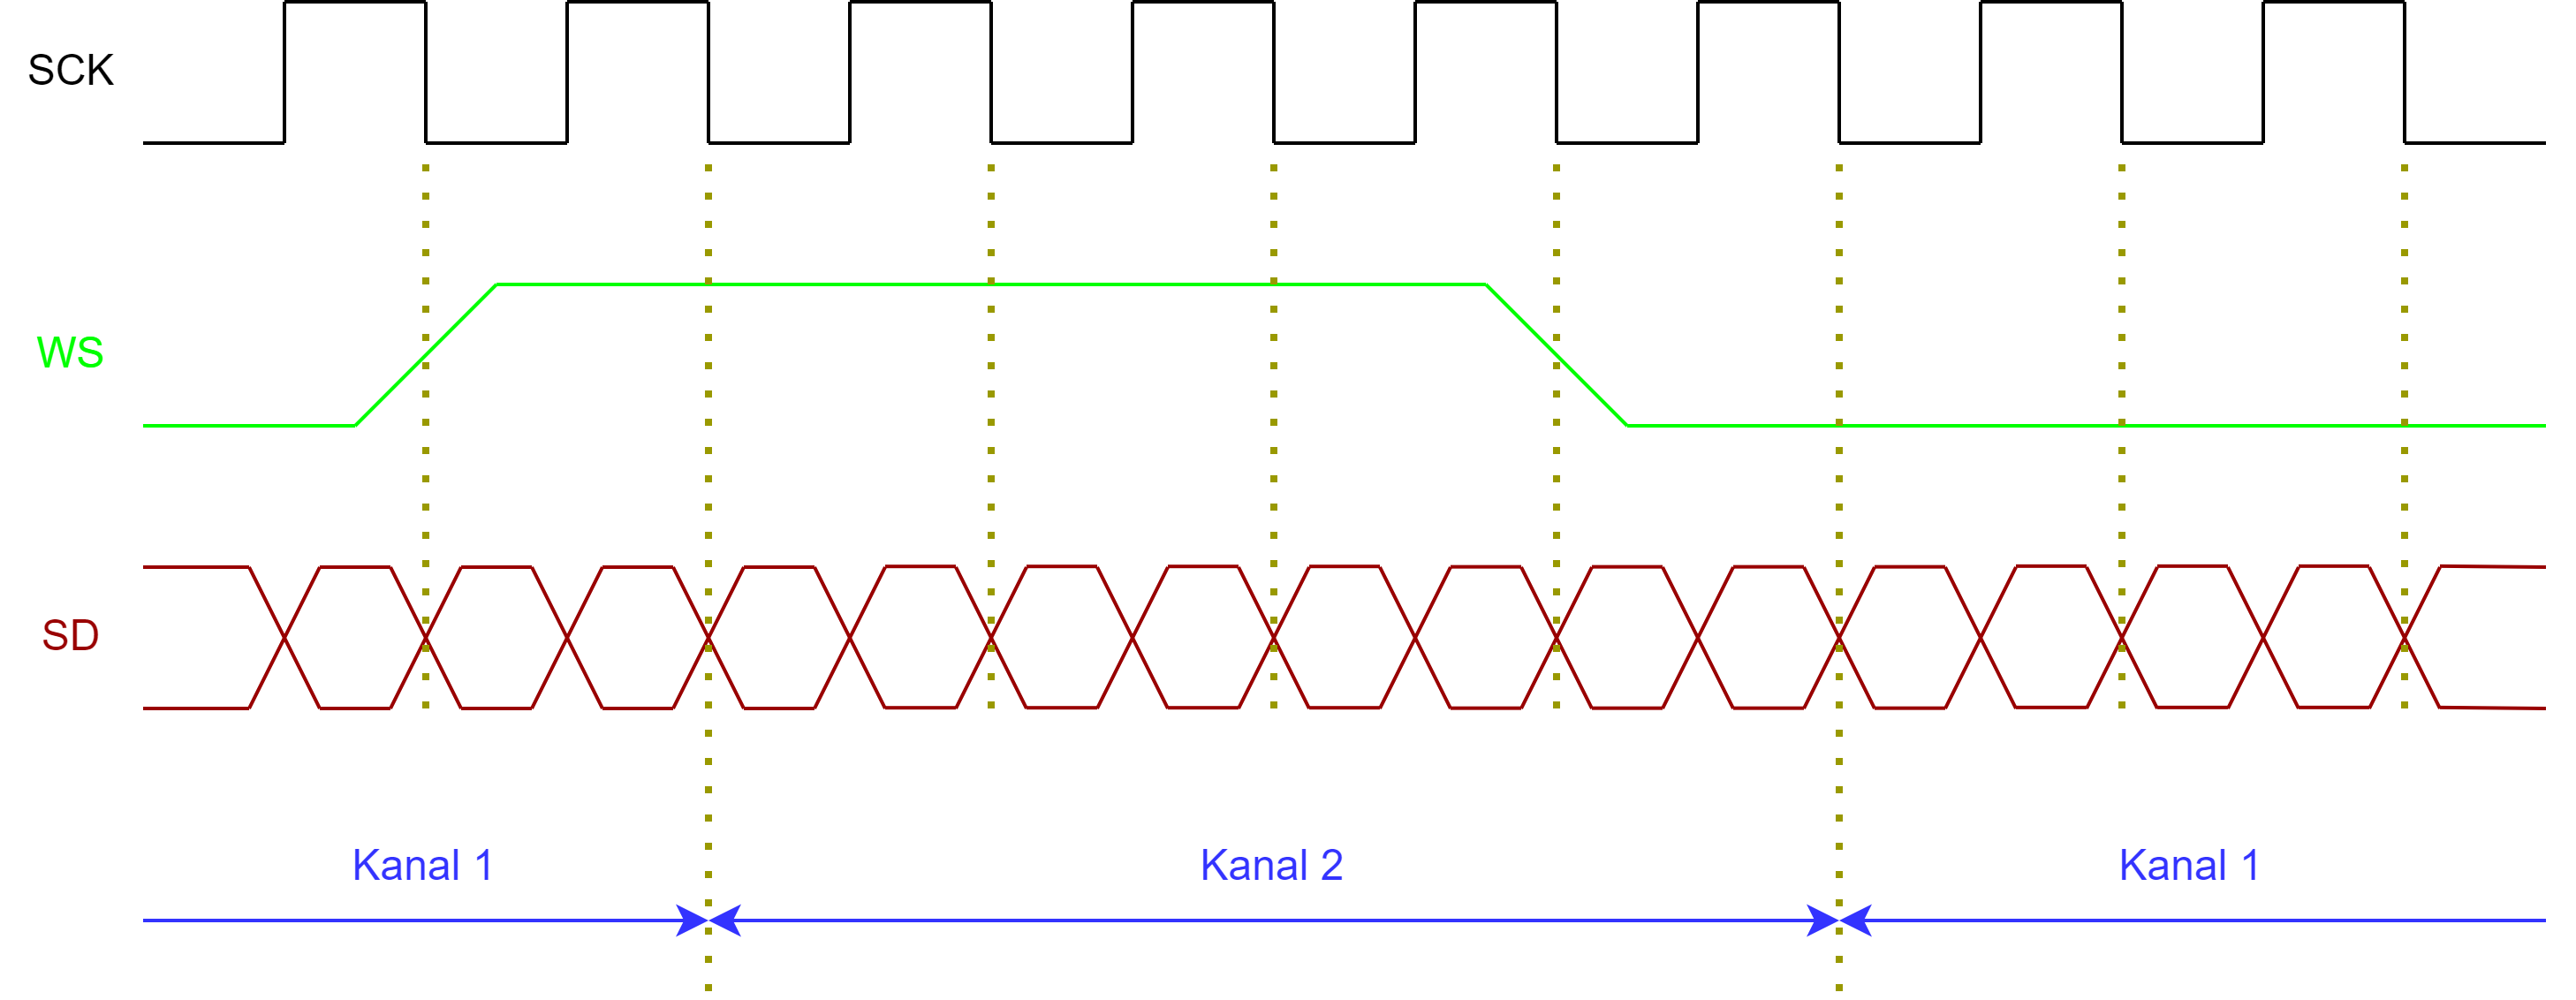
\includegraphics[width=1\linewidth]{images/BAT_I2S}
		\caption[]{Übersicht I2S-Signale}
		\label{fig:bati2s}
	\end{figure}
	
	\subsubsection{PDM}
	\subsubsection{Schalldruckpegel}
	\subsection{Komponentenwahl}
	\subsubsection{Kriterien}
	\subsubsection{Vergleich}
	
	\newpage
	\section{Mikrocontroller}
	\subsection{Grundlagen}
	\subsubsection{DMA}
	\subsubsection{BLE}
	\subsubsection{RTC}
	\subsubsection{Peripherie in Hardware oder Software}
	\subsection{Komponentenwahl}
	Es existieren eine Vielzahl von Mikrocontroller-Herstellern. Viele dieser verfügen über eine breite Palette an BLE-tauglichen Chips. Um den geeignetsten darunter zu finden, werden nachfolgend die benötigten Schnittstellen definiert und mehrere, vorselektionierte Mikrocontroller, miteinander verglichen.
	\subsubsection{Kriterien}
	\subsubsection{Vergleich}
	\subsubsection{Fazit}
	
	\newpage
	\section{LED}
	\subsection{Grundlagen}
	\subsubsection{Leistungsaufnahme}
	\subsubsection{Lichtleistung}
	\subsection{Komponentenwahl}
	\subsubsection{Kriterien}
	\subsubsection{Vergleich}
	
	\newpage
	\section{Entwicklung}
	\subsection{Hardware}
	\subsubsection{PCB}
	\subsubsection{Kosten}
	\subsection{Software}
	
	\newpage
	\section{Messungen}
	\subsection{Leistungsaufnahme}
	\subsection{Mikrofon-Kalibrierung}
	\subsection{Vergleich}
	
	\newpage
	\section{Fazit und Ausblick}
	
	\newpage
	\section{Anhang}
	
	
	
	
\end{document}